\section{Plug and Process Loads}
\label{sec:plug_and_process_loads}

Plug and process loads (PPLs) are all electrical or gas building loads that do not fall under lighting, heating, cooling, ventilation, or water heating. As lighting and HVAC equipment becomes more efficient, PPLs represent an increasing percentage of commercial building energy consumption---up to 50\% in high-performance buildings. This section describes how electric equipment, gas equipment, data centers, elevators, and kitchen equipment are modeled in ComStock. 

\subsection{Electric Equipment}

Electric equipment is a broad category that encompasses any type of load that is powered by an AC outlet. This can include computers, monitors, printers, kitchen or bathroom appliances, laundry equipment, phone chargers, and more. Because there are so many types of electric equipment, ComStock does not model each technology separately, but instead uses an equipment power density (EPD) value for each space type, in watts per square foot. 

The EPDs are derived from the DOE prototype buildings; however, some of the values were adjusted during the end-use load profiles calibration process. Using end-use-level data provided by two industry sources for a variety of building types, we increased or decreased some EPD assumptions to better reflect the actual building data. Building types that were affected by the EPD adjustments included Full Services Restaurant (FullServiceRestaurant), Primary School (PrimarySchool), Quick Service Restaurant (QuickServiceRestaurant), Retail (Retail), Secondary School (SecondarySchool), and Strip Mall (StripMall). 

The EPDs are dependent on building type, space type, and DOE Reference Building template. The interior equipment template is a function of the vintage of the building, as well as equipment turnover assumptions. In most cases, the EPD remains constant for all templates; however, some values increase or decrease in newer templates. An increase in the EPD in newer templates for a particular space type most likely indicates that new types of plug loads or technologies are assumed to be in the space. By comparison, a decrease in EPD indicates that plug loads in that space have become more efficient as buildings upgrade to newer equipment. For example, EPDs in the ``MediumOffice - Conference'' space type decrease beginning with the 90.1-2004 template, reflecting an assumption that conference equipment such as projectors and monitors have become more efficient. On the other hand, EPDs in ``MediumOffice - Breakroom'' increase drastically, likely due to the addition of new kitchen appliances and accessories. 

The EPDs in the ComStock model for each combination of building type, space type, and template are shown in Table ~\ref{tab:epds}.


\subsection{Gas Equipment}

Gas equipment refers to any natural gas-powered interior equipment that is not used for space heating or water heating. Similar to electric equipment, there are many different types of gas equipment, so ComStock does not model each technology individually, but rather uses a gas intensity in BTU per hour per square foot. Gas kitchen equipment makes up the majority of the gas equipment modeled in ComStock. Kitchen equipment will be discussed separately in Section 4.6.5. There are only three non-kitchen space types in our models that contain non-zero gas equipment values, and the values used are shown in Table~\ref{tab:gas_equip}. 

\begin{table}
\small
\centering
\caption[Gas Equipment Power Density]{Gas Equipment Power Density (Btu/hr*ft\textsuperscript{2})}
\label{tab:gas_equip}
\begin{tabular}{|l|l|r|r|r|r|r|r|}
\hline
\multicolumn{2}{|c|}{} & \multicolumn{6}{c|}{{\textbf{Template}}} \\ \hline
\textbf{Building Type} & \textbf{Space Type} & \textbf{Pre-1980} & \textbf{1980--2004} & \textbf{90.1-2004} & \textbf{90.1-2007} & \textbf{90.1-2010} & \textbf{90.1-2013} \\ \hline
LargeHotel & Laundry  & 170.0 & 170.0 & 170.0 & 170.0 & 170.0 & 170.0 \\ \hline
Outpatient & OR      & 23.9 & 23.9 & 23.9 & 23.9 & 23.9 & 23.9 \\ \hline
SmallHotel & Laundry  & 58.4 & 58.4 & 129.9 & 129.9 & 129.9 & 129.9 \\ \hline
\end{tabular}
\end{table}

The space types that contain gas equipment are the laundry and operating room space types in hotels and outpatient buildings, respectively. Gas laundry equipment represents gas clothes dryers, which are common in commercial drying applications. In operating rooms, a small amount of gas equipment represents steam sterilizers or autoclaves, which are used for sterilization during surgical procedures.

\subsection{Data Centers}

Data centers are a high-intensity type of PPL that house IT and computing equipment. Large standalone data centers are not currently modeled in ComStock, but this building type may be added in the future. Instead, ComStock models data centers as a space type within large and medium office buildings. This is meant to represent an IT closet or high-performance computer that is located within an office building and used by a business or organization. 

The data center is divided into two space types---a core data center and an IT closet. The core data center represents about 96\% of the data center floor area and has an equipment power density of 45 W/ft\textsuperscript{2}. The IT closet represents the remaining 4\% of the data center floor area and has an equipment power density of 20 W/ft\textsuperscript{2}. The area-weighted equipment power density of the whole data center is 44 W/ft\textsuperscript{2}, which is approximately 20--50 times the equipment load of most other space types \citep{osti_1129366}.

In the DOE large office prototype model, the data center represents 2.5\% of the total floor area. The medium office prototype model does not contain a data center space type. If we used the exact space type ratios from the prototype models for ComStock, all large offices would contain a data center, but no medium or small offices would contain this space type. In reality, not all office buildings contain data centers, and they can be present in offices of different sizes. Therefore, ComStock models data centers in a portion of large and medium office buildings. To determine these distributions, we used CBECS 2012 data to understand how prevalent data centers are in office buildings of different sizes. In addition, we used CBECS responses to determine what percent of a typical office building's floor area is dedicated to the data center. From this analysis, we decided that 38\% of large offices and 20\% of medium offices should contain data centers. In buildings with data centers, that space should make up approximately 2\% of the total square footage of the building. We also determined that data centers are uncommon in small offices; therefore, there is no data center space type in the small office models. 

Data centers follow a very different schedule than the rest of a building's plug and process loads. This type of IT equipment often runs 24 hours a day; therefore, the data center space type has a constant schedule year round. The start and stop time and base-to-peak ratio (BPR) schedule adjustments do not affect the data center space type. 

\subsection{Elevators}
Elevators are a high power density equipment load present in many commercial buildings. According to the Americans with Disabilities Act (ADA), elevators are required in all commercial buildings with three or more stories, or when the square footage of each floor is more than 3,000 square feet. Although not a requirement, many two-story buildings also contain elevators for accessibility and convenience. Therefore, ComStock includes elevators in all buildings with two or more stories.

Hydraulic elevators are assumed to be installed in buildings with two to six stories, and traction elevators are assumed to be installed in buildings taller than six stories. Hydraulic elevators use a fluid-driven piston to lift the cab, and typically operate at speeds of 150 feet per minute or less. Hydraulic elevators are more affordable and can carry heavier loads, but because of their slow speeds, they are typically only used in buildings up to five stories. For buildings with six or more stories, traction elevators are used because they operate at much higher speeds (up to 500 feet per minute). Traction elevators use a counterweight and pulley system, making them more energy efficient because the motor does not have to move as much weight. The drawbacks, however, include high installation and maintenance costs and limits on cab weights. The motor power is assumed to be 16,055 W for hydraulic elevators and 20,370 W for traction elevators. 

Elevators are modeled as a zone load in EnergyPlus, meaning the elevator equipment load and associated heat gain are attributed to a thermal zone. Elevator load is reported out as part of the electric equipment end use. With hydraulic elevators, the elevator room is typically located in the basement, so the equipment load and heat gain are added to the first floor core zone. With traction elevators, the elevator equipment is located on the roof, so the equipment load and heat gain are added to the top floor core zone.

The number of elevators installed in a ComStock building depends on the building type. For most building types, the number of elevators is based on the floor area. The exceptions are hospitals and hospitality buildings, for which assumptions are based on the number of hospital beds or hotel rooms, respectively. ComStock differentiates between passenger elevators and freight elevators in order to properly capture the elevator load in certain building types with industrial or service elevators. Passenger elevators are modeled in all building types, whereas freight elevators are only modeled in hospital, large hotel, large office, and warehouse buildings. The assumptions for the number of passenger and freight elevators modeled by building type are shown in Tables ~\ref{tab:passenger_elevators} and ~\ref{tab:freight_elevators}.

The equipment schedule for elevators is irregular and unpredictable. Therefore, this load does not follow the typical plug load schedule for its associated space type. We decided to approximate an elevator's schedule by relating it to the number of people who are entering or exiting the building at each time step---in other words, the derivative of the occupancy schedule of the building. We also made assumptions regarding the number of people per elevator ride (five), the amount of time per ride (calculated from the elevator speed and number of stories), and the amount of inter-floor traffic that is not captured by the change in building occupancy (added a factor of 1.2x). Elevator data and metrics like this are not commonly measured or available, so these assumptions are based primarily on engineering judgment. 

From these calculations and assumptions, we derived an elevator schedule for each building type and each day of the week. An example of the elevator schedule for medium offices is shown in Figure~\ref{fig:medium_office_elevator_schedule} for weekdays, Saturdays, and Sundays. On weekdays, the most elevator traffic occurs at the beginning and end of the day, when people are coming in or leaving work for the day. There is also significant traffic during the lunch hour, as some people choose to leave the building for lunch. At all other times during the workday, the elevator load is approximately 40\% of the total load to account for inter-floor traffic and minimal change in the total building occupancy. For some buildings, the occupancy schedules are reduced on Saturdays and include no occupancy on Sundays, which is reflected in the elevator schedule. 

\begin{figure}[ht!]
    \centering 
    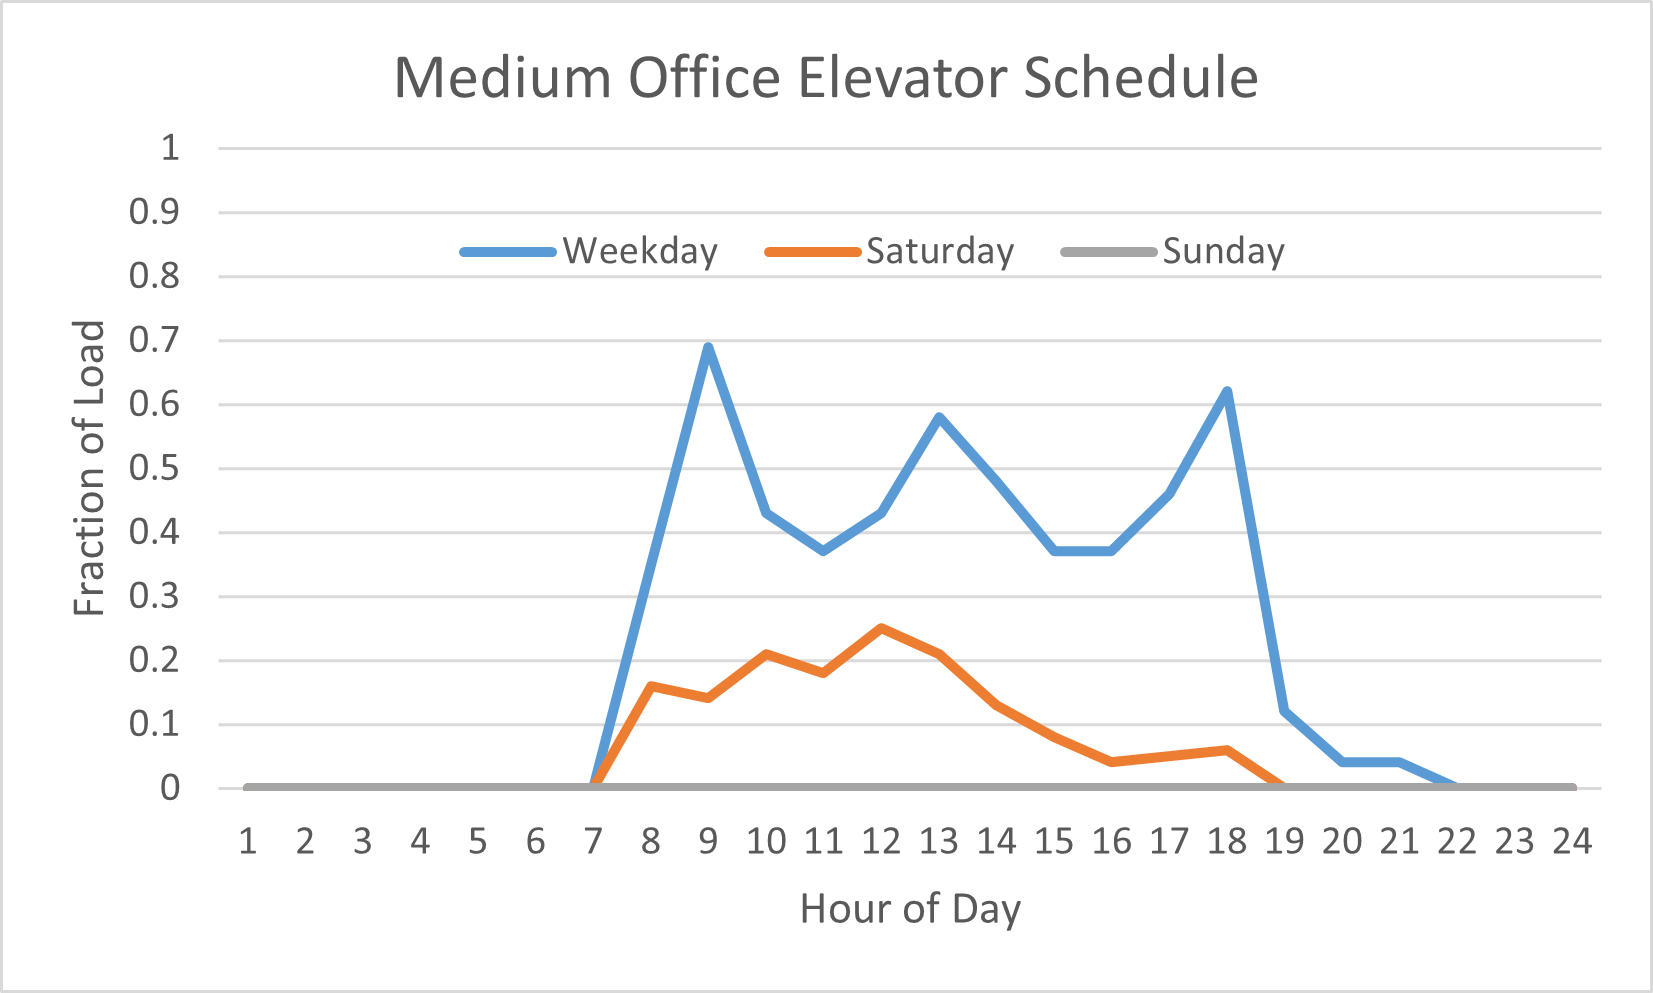
\includegraphics[]{figures/medium_office_elevator.png}
    \caption[Medium office elevator schedule]{Elevator fractional load schedule for medium offices on weekdays, Saturdays, and Sundays.}
    \label{fig:medium_office_elevator_schedule}
\end{figure}

The final aspect of modeling elevators is accounting for lighting and fans inside the elevator. Although these are minimal loads compared to the total elevator energy, they are still modeled in ComStock. The elevator lighting and fans are defined in the model by a total power in watts. These wattage values were calculated based on the number of elevators and the subsystem template in the model, thereby ensuring higher efficiencies for newer lighting and ventilation systems. The elevator lighting and fan schedules are assumed to be at full load at all times when the elevator schedule is greater than 0.

\pagebreak

\subsection{Kitchen Equipment} 
Kitchens are one of the most energy-intensive space types. In ComStock, kitchen space types are modeled in six building types---FullServiceRestaurant, Hospital, LargeHotel, PrimarySchool, QuickServiceRestaurant, and SecondarySchool. In some building types, namely restaurants, the kitchen space type represents a significant proportion of the floor area. In these cases, kitchen loads have a major impact on the total building EUI. In hotels, hospitals, and schools, the kitchen space type only represents a small fraction of the total floor area. Table~\ref{tab:kitchen_floor_area} shows the percent of the total floor area represented by the kitchen space type for each building type. Note that some of the strip malls in ComStock contain some fraction of the "QuickServiceRestaurant" building type to account for food service that is often found in strip malls. 

\begin{table}[h!]
\small
\centering
\caption[Kitchen Space Type Percentage of Total Floor Area]{Kitchen Space Type Percentage of Total Floor Area}
\label{tab:kitchen_floor_area}
\begin{tabular}{|l|l|l|}
\hline
\textbf{Building Type}          & \textbf{Space Type} & \textbf{Percentage of Total Floor Area} \\ \hline
FullServiceRestaurant  & Kitchen    & 27.3\%                         \\ \hline
Hospital               & Kitchen    & 4.1\%                          \\ \hline
LargeHotel             & Kitchen    & 0.9\%                          \\ \hline
PrimarySchool          & Kitchen    & 2.4\%                          \\ \hline
QuickServiceRestaurant & Kitchen    & 50\%                           \\ \hline
SecondarySchool        & Kitchen    & 1.1\%                          \\ \hline
\end{tabular}
\end{table}

Commercial building energy modeling often assumes an energy intensity per area for cooking equipment, like what is used in the DOE prototype buildings (\cite{qsr_50pct_svs}). However, applying these power densities directly to the various building sizes in ComStock assumes cooking loads scale linearly with kitchen square footage, which does not necessarily represent reality (\cite{eia2012cbecs},~\cite{qsr_50pct_svs}). Further, it does not allow for straightforward analysis of specific cooking equipment since it is represented by a single aggregate load. However, little information exists regarding representative equipment-specific modeling of cooking appliances, as well as how cooking equipment scales with building area. The CBECS survey does provide some level of guidance for area-based intensity as they disaggregate cooking energy consumption separately and provide building area for their samples, but this end use energy consumption data is derived using statistical means from monthly billing data rather than directly measured making it less reliable (\cite{eia2012cbecs},~\cite{qsr_50pct_svs}).


ComStock uses published data to create representative probability distributions of commercial cooking equipment counts, by building type, for both gas and electric appliances. Additionally, the equipment distributions are scaled by area to represent the non-linear scaling suggested in the literature. Although other building types likely include some degree of cooking equipment as well, such as larger offices (\cite{eia2012cbecs}), the current implementation of ComStock only includes cooking equipment in the previously-mentioned six building types plus quick service restaurants found in strip malls. 

Commercial kitchens can contain electric or gas cooking equipment, or a mix of both. The prevalence of gas and electric fuel types for each equipment type and the rated powers used in ComStock are derived from a DOE study (\cite{goetzler_commercial_appliances}). These are shown in Table~\ref{tab:kitchen_prev_and_power}. 

% Please add the following required packages to your document preamble:
% \usepackage{multirow}
% \usepackage{graphicx}
\begin{table}[]
    \caption[Cooking Equipment Fuel Type Prevelance and Rater Power]{Cooking Equipment Fuel Type Prevelance and Rater Power}
    \label{tab:kitchen_prev_and_power}
    \resizebox{\columnwidth}{!}{%
    \begin{tabular}{|l|ll|ll|ll|ll|ll|}
    \hline
    \multicolumn{1}{|c|}{\multirow{2}{*}{\textbf{Appliance}}} &
      \multicolumn{2}{c|}{\textbf{Fuel Prevalence Fraction}} &
      \multicolumn{2}{c|}{\textbf{Rated Power}} &
      \multicolumn{2}{c|}{\textbf{Fraction Radiant}} &
      \multicolumn{2}{c|}{\textbf{Fraction Latent}} &
      \multicolumn{2}{c|}{\textbf{Fraction Lost}} \\ \cline{2-11} 
    \multicolumn{1}{|c|}{} &
      \multicolumn{1}{l|}{\textbf{Gas}} &
      \textbf{Electric} &
      \multicolumn{1}{l|}{\textbf{Gas (Btu/h)}} &
      \textbf{Electric (kW)} &
      \multicolumn{1}{l|}{\textbf{Gas}} &
      \textbf{Electric} &
      \multicolumn{1}{l|}{\textbf{Gas}} &
      \textbf{Electric} &
      \multicolumn{1}{l|}{\textbf{Gas}} &
      \textbf{Electric} \\ \hline
    Broiler &
      \multicolumn{1}{l|}{0.91} &
      0.09 &
      \multicolumn{1}{l|}{96,000} &
      10.8 &
      \multicolumn{1}{l|}{0.12} &
      0.35 &
      \multicolumn{1}{l|}{0.1} &
      0.1 &
      \multicolumn{1}{l|}{0.68} &
      0.45 \\ \hline
    Griddle &
      \multicolumn{1}{l|}{0.58} &
      0.42 &
      \multicolumn{1}{l|}{90,000} &
      17.1 &
      \multicolumn{1}{l|}{0.18} &
      0.39 &
      \multicolumn{1}{l|}{0.1} &
      0.1 &
      \multicolumn{1}{l|}{0.62} &
      0.41 \\ \hline
    Fryer &
      \multicolumn{1}{l|}{0.5} &
      0.5 &
      \multicolumn{1}{l|}{80,000} &
      14 &
      \multicolumn{1}{l|}{0.23} &
      0.36 &
      \multicolumn{1}{l|}{0.1} &
      0.1 &
      \multicolumn{1}{l|}{0.57} &
      0.44 \\ \hline
    Oven &
      \multicolumn{1}{l|}{0.55} &
      0.45 &
      \multicolumn{1}{l|}{44,000} &
      12.1 &
      \multicolumn{1}{l|}{0.08} &
      0.22 &
      \multicolumn{1}{l|}{0.1} &
      0.1 &
      \multicolumn{1}{l|}{0.72} &
      0.58 \\ \hline
    Range &
      \multicolumn{1}{l|}{0.91} &
      0.09 &
      \multicolumn{1}{l|}{145,000} &
      21 &
      \multicolumn{1}{l|}{0.11} &
      0.1 &
      \multicolumn{1}{l|}{0.1} &
      0.1 &
      \multicolumn{1}{l|}{0.69} &
      0.7 \\ \hline
    Steamer &
      \multicolumn{1}{l|}{0.33} &
      0.67 &
      \multicolumn{1}{l|}{200,000} &
      27 &
      \multicolumn{1}{l|}{0.1} &
      0.1 &
      \multicolumn{1}{l|}{0.1} &
      0.1 &
      \multicolumn{1}{l|}{0.7} &
      0.7 \\ \hline
    \end{tabular}%
    }
    \end{table}

Kitchens in ComStock models are assigned a quantity of each equipment type. These can be found in the ComStock metadata files for each model. Equipment quantities are assigned using probability distribtuions with dependencies on building type and food service floor area. The quantities used in the probability distributions are determined using an older dataset of equipment counts per restaurant type combined with the prevalence of the restaurant type (\cite{com_food_service_equip}). The restaurant types were mapped to ComStock building types. This is summarized in Table~\ref{tab:kitchen_cook_counts}. Unfortunately, little data of this type was found in literature, so this older source was ultimately used for equipment counts. However, even with changes in culinary trends, it is not expected that counts of equipment types in a restaurant would have changed drastically over the past few decades. Additionally, a “None” restaurant type was created for schools, with a prevalence determined by the fraction of schools in CBECS that have kitchens (\cite{eia2012cbecs}).

This workflow also includes modifiers to the equipment counts shown in Table~\ref{tab:kitchen_cook_counts} to scale equipment count for different kitchen sizes. As mentioned previously, it is not expected that equipment scales linearly with kitchen size, but there is little information in the literature to suggest appropriate scaling (\cite{qsr_50pct_svs}). To account for equipment count scaling, we assume most typically-sized kitchens will have the same quantity of equipment. However, especially small and large kitchens will include scaling factors to account for very large changes in kitchen area that would likely correlate to higher/lower meals served. These factors were determined using engineering judgment and are summarized in Figure~\ref{fig:cooking_equipment_count_scaling_factors_by_building_type_and_area}.

In summary, ComStock determines quantity and fuel type of cooking equipment based on sampling our probability distributions. A restaurant type is sampled for each model as per the prevenances shown by building type in Table~\ref{tab:kitchen_cook_counts}. This yields the corresponding equipment counts for the restaurant type shown in Table~\ref{tab:kitchen_cook_counts}, with square footage modifiers applied based on building size and type. Next, the equipment fuel type is sampled as per the prevalence shown in Table~\ref{tab:kitchen_prev_and_power} for each piece of equipment. Combined, this yields quantities of gas and electric cooking equipment for each ComStock sample. Note that kitchen spaces in ComStock additionally include some prevalence of electric load to account for non-major electrical appliances such as microwaves, heating lamps, toasters, coffee machines, electric kettles, etc. Additionally, the current implementation of cooking equipment in ComStock utilizes the same schedule for each equipment type. Future work could include implementing equipment-specific schedules for the various equipment types, which may better represent reality.


\begin{figure}[ht!] \centering 
    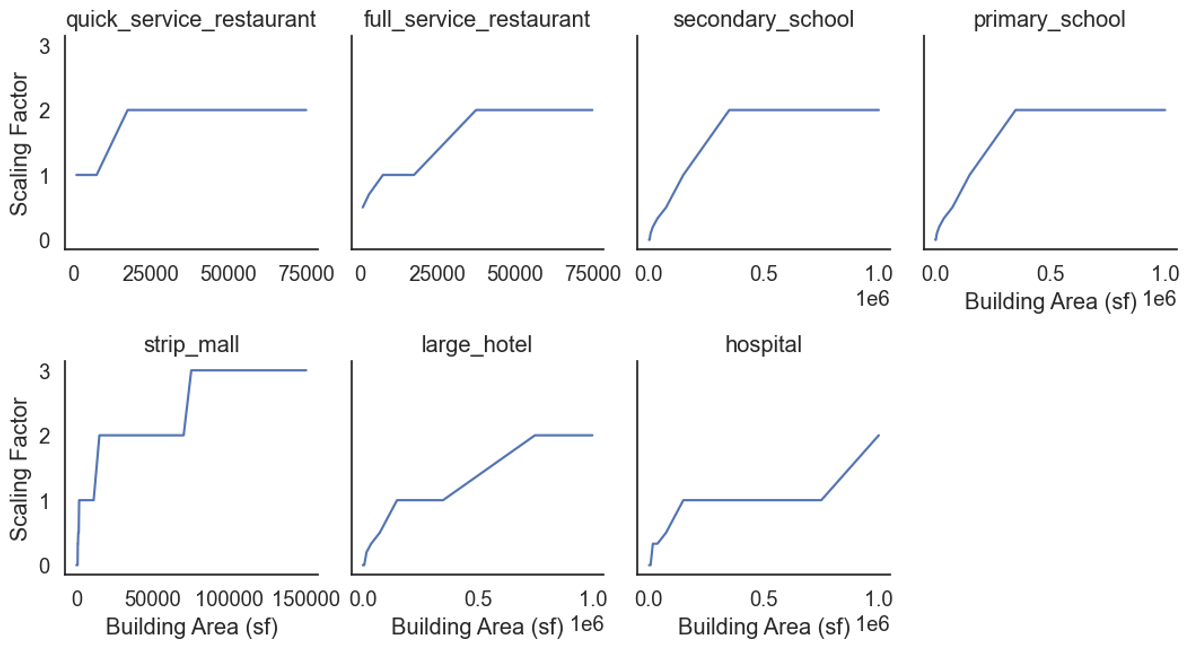
\includegraphics[
        page={1},
        %trim={1cm 18.3cm 1cm 1cm}, clip, % L B R T
        width=\textwidth]{figures/kitchen_equipment_count_scaling.png}
    \caption[Cooking equipment count scaling factors by building type and area]{Cooking equipment count scaling factors by building type and area.}
    \label{fig:cooking_equipment_count_scaling_factors_by_building_type_and_area}
\end{figure}
